\chapter{گام 1: شناسایی توالی های بالقوه زایلاناز}
    اولین مرحله در این مطالعه شامل شناسایی توالی‌های متاژنومی است که به طور بالقوه آنزیم‌های زایلاناز مقاوم در برابر حرارت را رمزگذاری می‌کنند. این از طریق جستجوی مبتنی بر شباهت در برابر مجموعه‌ای از توالی‌های زایلاناز شناخته شده با استفاده از ابزارهای هم‌ترازی توالی محاسباتی به دست می‌آید. هدف اصلی فیلتر کردن contig هایی است که مشابهت قابل توجهی با زایلانازهای مرجع دارند و اطمینان حاصل شود که فقط مرتبط ترین توالی ها برای تجزیه و تحلیل بیشتر حفظ می شوند.

    \section*{رویکرد: جستجوی شباهت با استفاده از BLAST، DIAMOND، یا HMMER}
        برای شناسایی ژن های بالقوه کد کننده زایلاناز، از ابزارهای زیر استفاده می شود:
        \begin{itemize}
            \item \lr{BLAST+ 
            (Basic Local Alignment Search Tool)}: 
            یک الگوریتم مقایسه توالی پرکاربرد است که مناطق شباهت بین کانتیگ های متاژنومی و توالی های زایلاناز شناخته شده را شناسایی می کند.
            \item DIAMOND : جایگزین سریع‌تری برای BLAST، بهینه‌سازی شده برای داده‌های متاژنومی در مقیاس بزرگ، که می‌تواند به سرعت توالی‌ها را در مقابل پایگاه‌های داده پروتئینی تراز کند.
            \item HMMER (جستجوی مبتنی بر مدل مارکوف پنهان): ابزار احتمالی است که نقوش حفاظت شده و حوزه های عملکردی مشخصه آنزیم های زایلاناز را تشخیص می دهد.
        \end{itemize}

    {\Large در این پروژه ما برای تعیین شباهت از ‌BLAST استفاده می‌کنیم:}\\
    BLASTX به دلیل دقت بالای آن در تشخیص توالی های همولوگ انتخاب شد، در حالی که از DIAMOND برای پردازش سریعتر مجموعه داده های متاژنومی بزرگ استفاده می شود. HMMER برای تشخیص شباهت‌های مبتنی بر نمایه استفاده می شود، که به شناسایی همولوگ‌های راه دور کمک می‌کند که تنها با شباهت توالی ثبت نشده‌اند. آستانه‌های فیلتر فقط مطابق با اطمینان بالا حفظ می‌شوند و از انتخاب نامزد قابل اطمینان اطمینان می‌دهند.
    نحوه عملکرد BLAST:
    \begin{enumerate}
        \item دنباله ورودی را می‌گیرد.(دنباله‌ای از DNA, RNA یا پروتیین‌‌ها)
        \item به دنبال دنباله‌‌های مشابه در دنباله‌های شناخته شده و پایگاه داده می‌گردد.
        \item محاسبه معیار شباهت
    \end{enumerate}

    \section{دستورات ترمینال برای شناسایی توالی}
        \begin{enumerate}
            \item نصب ابزار های مورد نیاز:
                \begin{figure}[H]
                    \centering
                    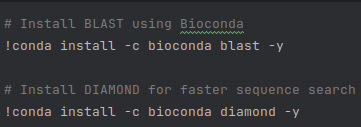
\includegraphics[width=0.5\textwidth]{images/install_blast.jpg} % Replace with your image file
                    \caption{نصب ابزار های مورد نیاز}
                    \label{fig:install_blast}
                \end{figure}
            \item  آماده سازی پایگاه داده BLAST:\\
                با اجرای این دستور در ترمینال از روی فایل (۱۱ دنباله‌ی شناخته شده زایلاناز) thermo\_xylanase.fasta فایل سازگار xylanase\_db ساخته می‌شود.
                \begin{figure}[H]
                    \centering
                    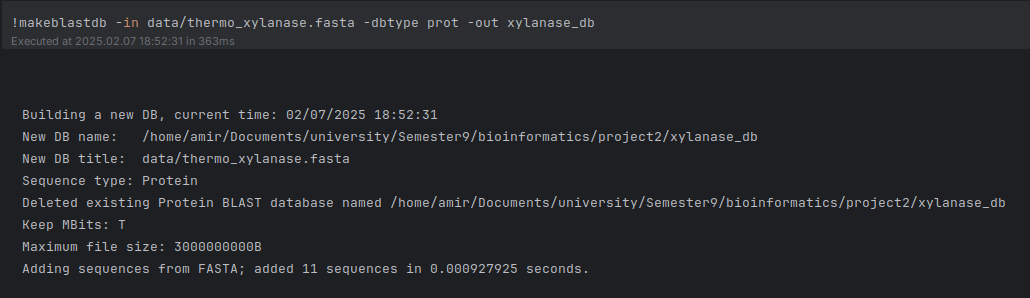
\includegraphics[width=0.7\textwidth]{images/blast_database.png} % Replace with your image file
                    \caption{آماده سازی پایگاه داده BLAST }
                    \label{fig:blast_database}
                \end{figure}

            \item اجرای BLASTX را برای شناسایی توالی های زایلاناز   بالقوه \\
                این دستور فایل تولید شده در قسمت قبل و پایگاه داده را گرفته و فایل نتایج (blast\_results.text) را با معیار شباهت(evalue) به مقدار 1e-5  تولید می‌کند.
                \begin{figure}[H]
                    \centering
                    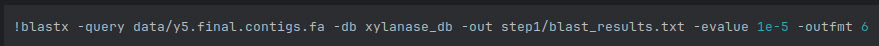
\includegraphics[width=0.8\textwidth]{images/run_blast.jpg} % Replace with your image file
                    \caption{آماده سازی پایگاه داده BLAST }
                    \label{fig:run_blast}
                \end{figure}
                

            \item \lr{blast\_results.txt}
                \begin{figure}[H]
                    \centering
                    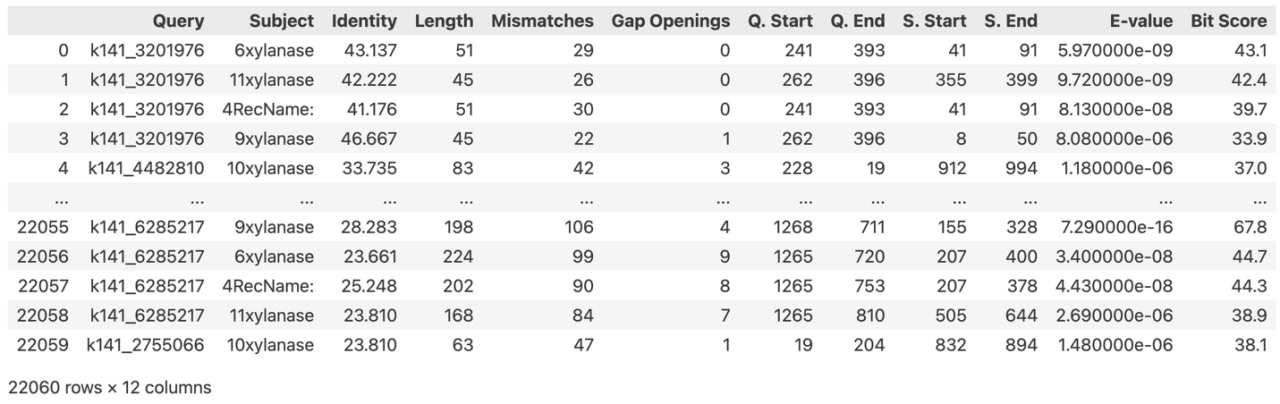
\includegraphics[width=0.8\textwidth]{images/blast_result.jpg} % Replace with your image file
                    \caption{نتیجه blast }
                    \label{fig:run_blast}
                \end{figure}
                \begin{table}[H]
                    \centering
                    \begin{tabular}{|c|c|c|}
                        \hline
                        1 & شناسایی توالی کوئری & k141\_2755066 \\
                        2 & شناسه توالی زایلاناز تطبیق‌یافته & 10xylanase \\
                        3 & درصد تطابق‌های یکسان & 23.810 \\
                        4 & طول ناحیه تطبیق‌یافته & 63 \\
                        5 & تعداد اسیدهای آمینه نامطابق & 47 \\
                        6 & تعداد شکاف‌های ایجادشده در هم‌ترازی & 1 \\
                        7 & موقعیت شروع در کانتیگ & 19 \\
                        8 & موقعیت پایان در کانتیگ & 204 \\
                        9 & موقعیت شروع در توالی زایلاناز & 832 \\
                        10 & موقعیت پایان در توالی زایلاناز & 894 \\
                        11 & مقدار معیار شباعت &  1.48e-06\\
                        12 & امتیاز کیفیت هم‌ترازی & 38.1 \\
                        \hline
                    \end{tabular}
                    \caption{Example Table}
                    \label{tab:example}
                \end{table}

            \item اجرای مشابه DIAMOND
                \begin{figure}[H]
                    \centering
                    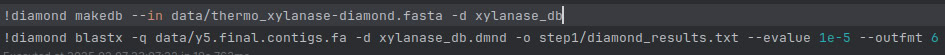
\includegraphics[width=0.8\textwidth]{images/run_diamond.jpg} % Replace with your image file
                    \caption{اجرای مشابه DIAMOND}
                    \label{fig:run_diamond}
                \end{figure}

        \end{enumerate}
        در مرحله بعد از بین دنباله‌های موجود در فایل نتایج تعدادی از آن‌ها را جدا می‌کنیم. در هنگامی که BLAST اجرا می‌شود معیار شباهت و امتیاز کیفینت همترازی برای هر رشته و رشته‌های موجود در دنباله‌های شناخته شده بدست می‌آيد. بر اساس این دو معیار دنباله‌‌های موجود در فایل نتایج فیلتر می‌شوند و دنباله‌هایی که همخوانی بیشتری با دنباله‌ی اصلی دارند بر گزیده خواهند شد.
    \subsubsection*{معیارهای انتخاب: آستانه تشابه}
        برای اطمینان از صحت شناسایی زایلاناز، توالی ها بر اساس معیارهای زیر فیلتر می شوند:
        \begin{enumerate}
            \item $E-value \le 1e-5$: (نشان دهنده شباهت آماری معنی دار).
            \item $\text{\lr{Percentage Identity}} \ge 30\%$ :(برای حفظ توالی هایی با سطح معنی داری از شباهت به زایلانازهای شناخته شده).
            \item $\text{\lr{Query Coverage}} \ge 50\%$ :(تضمین اینکه بخش قابل توجهی از contig با دنباله های مرجع همسو می شود).
        \end{enumerate}
        این آستانه‌ها حساسیت و ویژگی را متعادل می‌کنند و امکان تشخیص زایلانازهای نزدیک و بالقوه جدید را فراهم می‌کنند و در عین حال موارد مثبت کاذب را به حداقل می‌رسانند.

    \subsubsection*{فیلتر کردن:}
        \textbf{چرا نیاز است فیلتر انجام دهیم؟}\\
        BLASTX معیار شباهت را ارائه می دهد، اما به طور خودکار نتایج را فیلتر نمی کند. همه ترازهای بالاتر از یک آستانه مشخص را خروجی می دهد. با این حال، برخی از این تطابق‌ها ممکن است با اطمینان کم یا تطابق جزئی باشند، به این معنی که برای افزایش دقت به فیلتر دستی نیاز داریم.
        برخی از ترازها ممکن است دارای درصد کمی همترازی باشند (مثلاً 30-25٪) و ممکن است زایلاناز واقعی نباشند. ما باید یک برش تعیین کنیم تا فقط دنباله‌های مشابه‌ حفظ شوند. همچنین ترازهای کوتاه ممکن است کل پروتئین را پوشش ندهند. یک تطابق کوتاه (مثلاً 30 اسید آمینه از یک پروتئین 300 اسید آمینه) ممکن است شواهد کافی مبنی بر اینکه یک توالی آنزیم کامل زایلاناز را کد می کند، نباشد. فیلتر کردن بر اساس طول تراز به حذف این موارد کمک می کند.
        \begin{figure}[H]
            \centering
            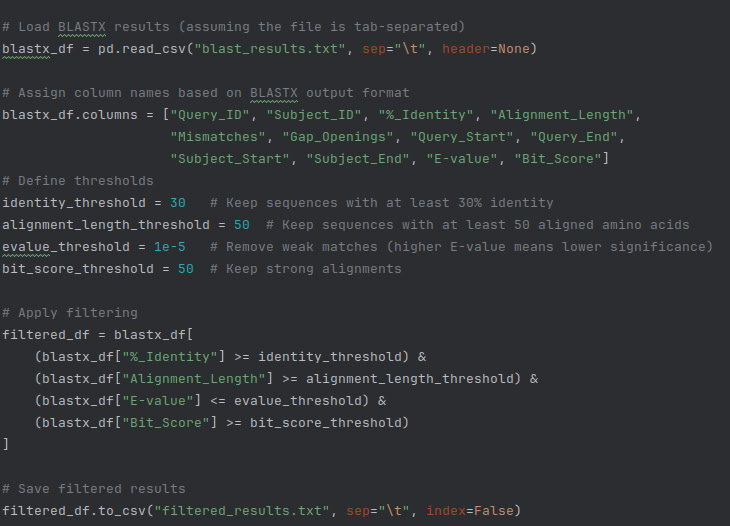
\includegraphics[width=0.8\textwidth]{images/step1_filter.jpg} % Replace with your image file
            \caption{فیلتر کردن.}
            \label{fig:step1_filter}
        \end{figure}
        \begin{figure}[H]
            \centering
            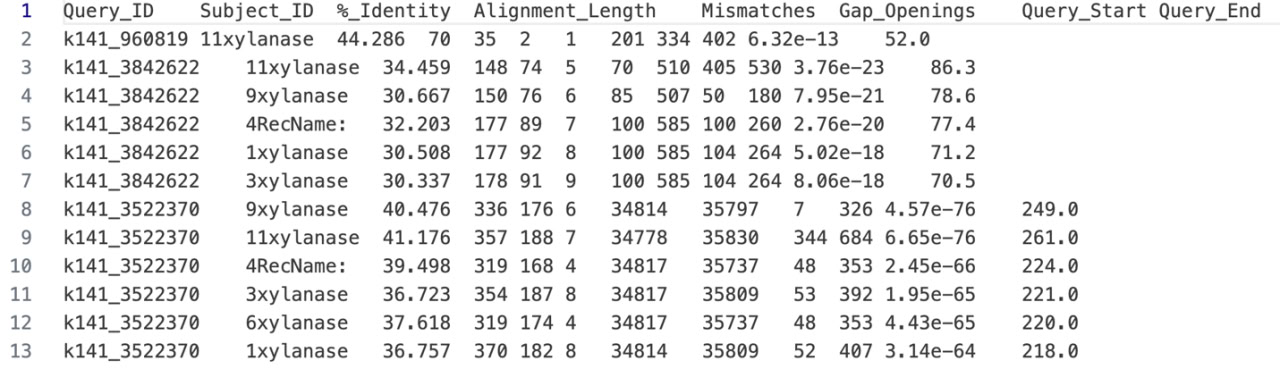
\includegraphics[width=0.8\textwidth]{images/filtered_results.jpg} % Replace with your image file
            \caption{filtered\_results.txt}
            \label{fig:filtered_results}
        \end{figure}
        \begin{figure}[H]
            \centering
            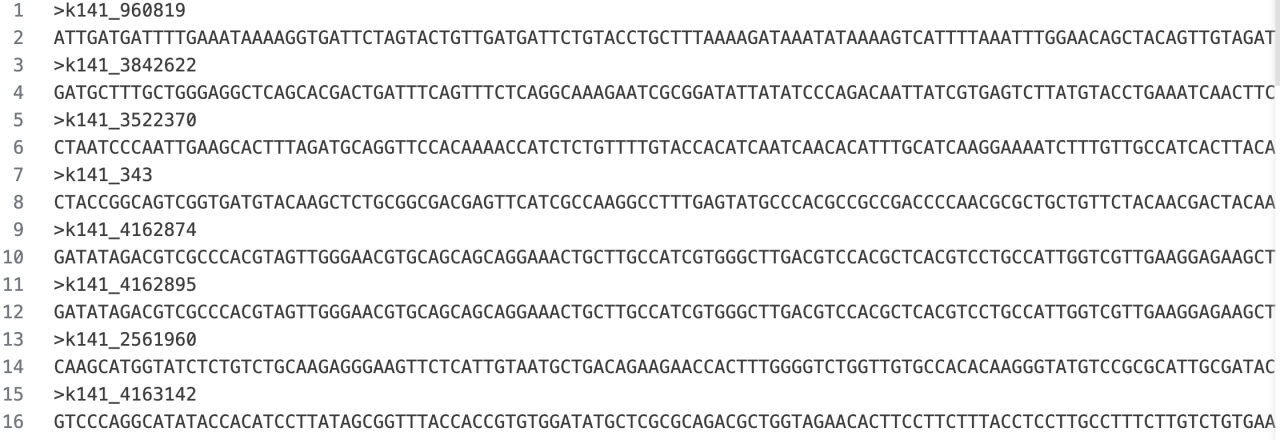
\includegraphics[width=0.8\textwidth]{images/filtered_contigs.jpg} % Replace with your image file
            \caption{filtered\_contigs.txt}
            \label{fig:filtered_contigs}
        \end{figure}
        آنچه BLASTX در واقع خروجی می دهد بخش منطبق از پیوند با یک پروتئین هماهنگ است. توالی کامل ترجمه شده contig را بر نمی گرداند. در این قسمت توالی کامل ترجمه کانتیگ را از پایگاه داده اصلی پیدا کرده و خروجی می‌دهیم.

    \subsubsection*{ترجمه کردن:}
        \begin{figure}[H]
            \centering
            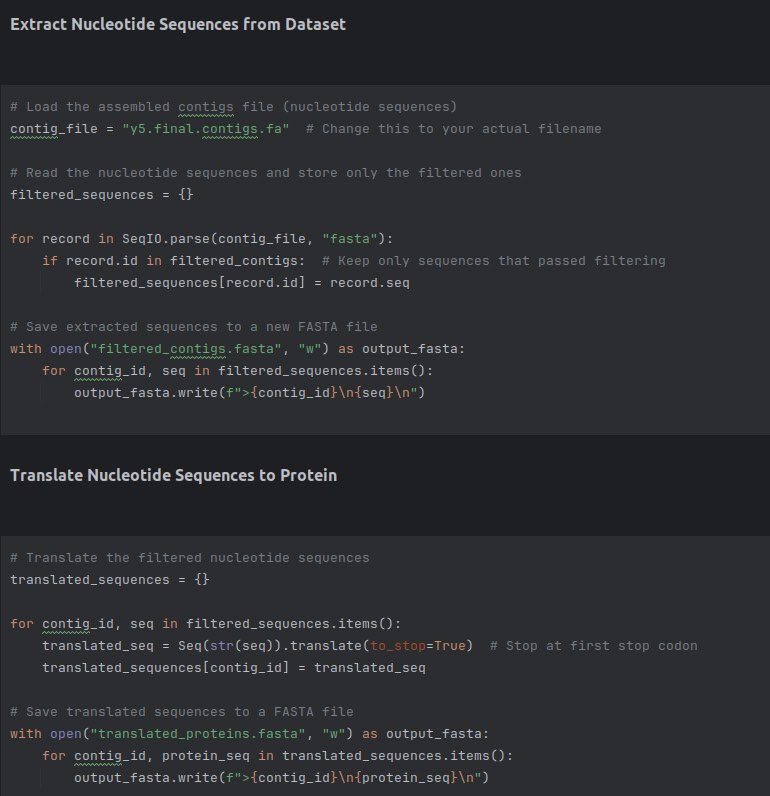
\includegraphics[width=0.8\textwidth]{images/step1_translate.jpg} % Replace with your image file
            \caption{ترجمه کردن.}
            \label{fig:step1_translate}
        \end{figure}
    \subsubsection*{ترجمه با استفاده از کامند ترمینال:}
        \begin{figure}[H]
            \centering
            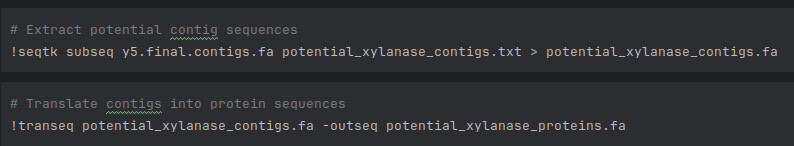
\includegraphics[width=0.8\textwidth]{images/step1_translate_terminal.jpg} % Replace with your image file
            \caption{ترجمه با استفاده از کامند ترمینال.}
            \label{fig:step1_translate_terminal}
        \end{figure}
    \subsection{تجزیه و تحلیل نتایج و نمودار های BLAST}
        \subsubsection{1. کلیت نتایج BLAST}
        تجزیه و تحلیل BLAST چندین پیوند را شناسایی کرد که با آنزیم های زایلاناز شناخته شده با درجات مختلف شباهت مطابقت داشتند. پارامترهای کلیدی مورد تجزیه و تحلیل عبارتند از:
        \begin{itemize}
            \item درصد هویت: شباهت بین پرس و جو و دنباله موضوع را اندازه می گیرد.
            \item امتیاز بیت: نمرات بالاتر نشان دهنده تراز قوی تر است.
            \item E-value: نشان دهنده اهمیت آماری است. مقادیر پایین تر نشان دهنده تطابق قابل اعتمادتر است.
        \end{itemize}
        \subsubsection{2. تفسیر نمودار ها}
        
        \begin{enumerate}[label=\alph*-]
            \item 
            \begin{figure}[H]
                \centering
                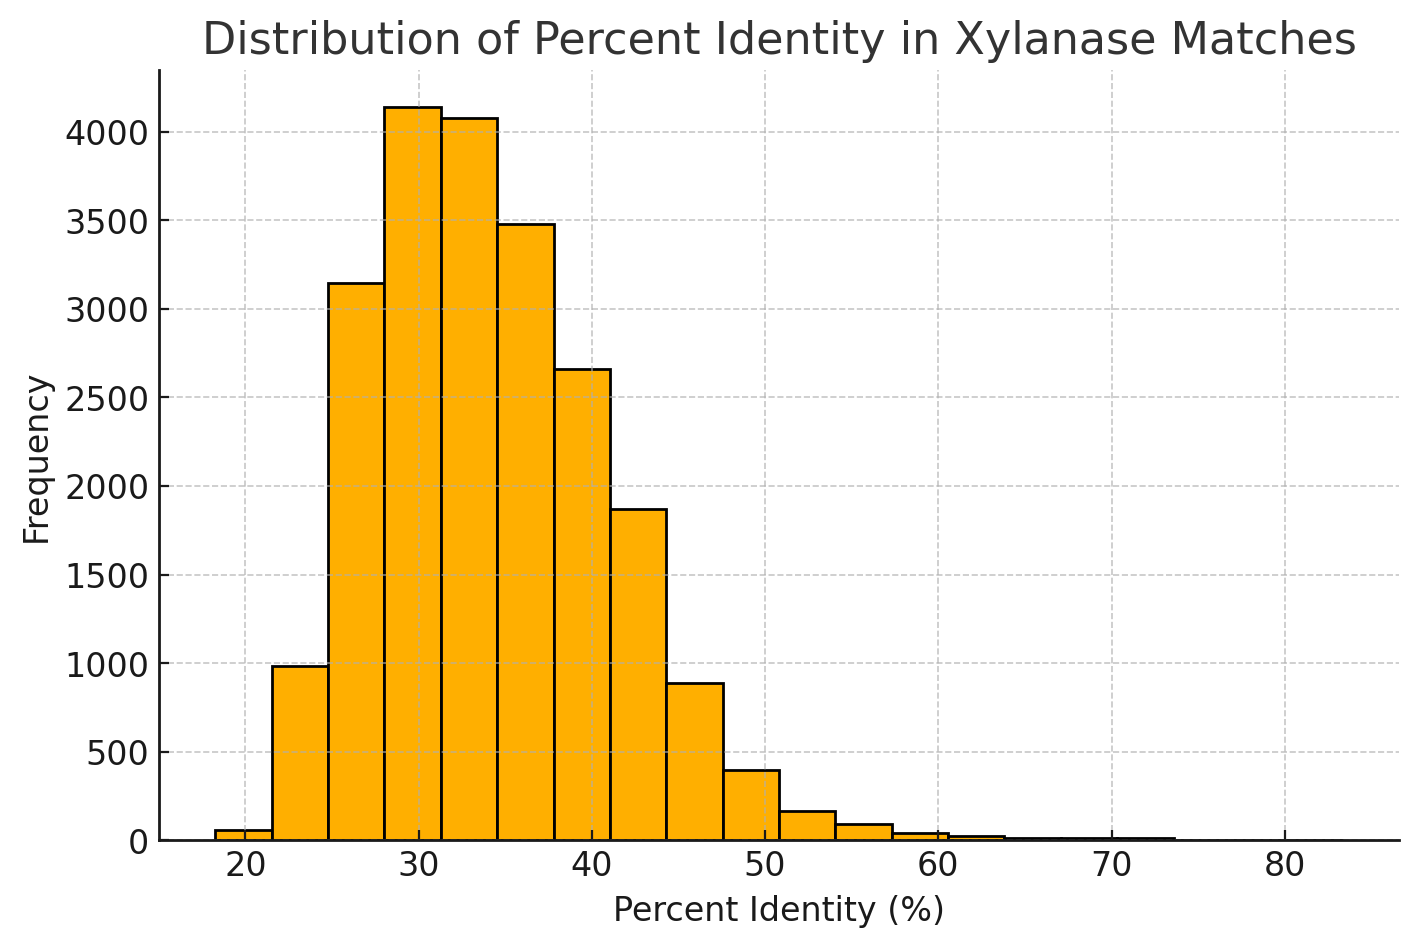
\includegraphics[width=0.8\textwidth]{images/dist_percent_identity.png} % Replace with your image file
                \caption{نمودار هیستوگرام درصد توزیع هویت.}
                \label{fig:dist_percent_identity}
            \end{figure}
            هیستوگرام: درصد توزیع هویت \\
            مشاهدات:
            \begin{itemize}
                \item توزیع طیف وسیعی از مقادیر هویت درصد را نشان می دهد.
                \item اکثر تطابق ها بین 
                30\% 
                و 
                50\%
                هویت قرار می گیرند، که نشان می دهد برخی از توالی های شناسایی شده ممکن است از فاصله دور با زایلانازهای شناخته شده مرتبط باشند.
                \item بخش کوچکتر دارای درصد هویت بالاتر 
                (> 50\%) 
                است که نشان دهنده روابط تکاملی قوی تر با زایلانازهای شناخته شده است.
            \end{itemize}
            مفاهیم:
            \begin{itemize}
                \item توالی های با هویت بالا (50-60\%) احتمالا زایلانازهای کاربردی با خواص بیوشیمیایی مشابه با آنزیم های شناخته شده هستند.
                \item توالی های با هویت پایین تر (30-40\%) ممکن است گونه های جدید زایلاناز را با پتانسیل برای کاربردهای بیوتکنولوژیکی نشان دهند.
                \item ممکن است برای تأیید فعالیت در توالی‌های با هویت پایین‌تر، تحلیل دامنه عملکردی بیشتری مورد نیاز باشد.
            \end{itemize}

            \item 
            \begin{figure}[H]
                \centering
                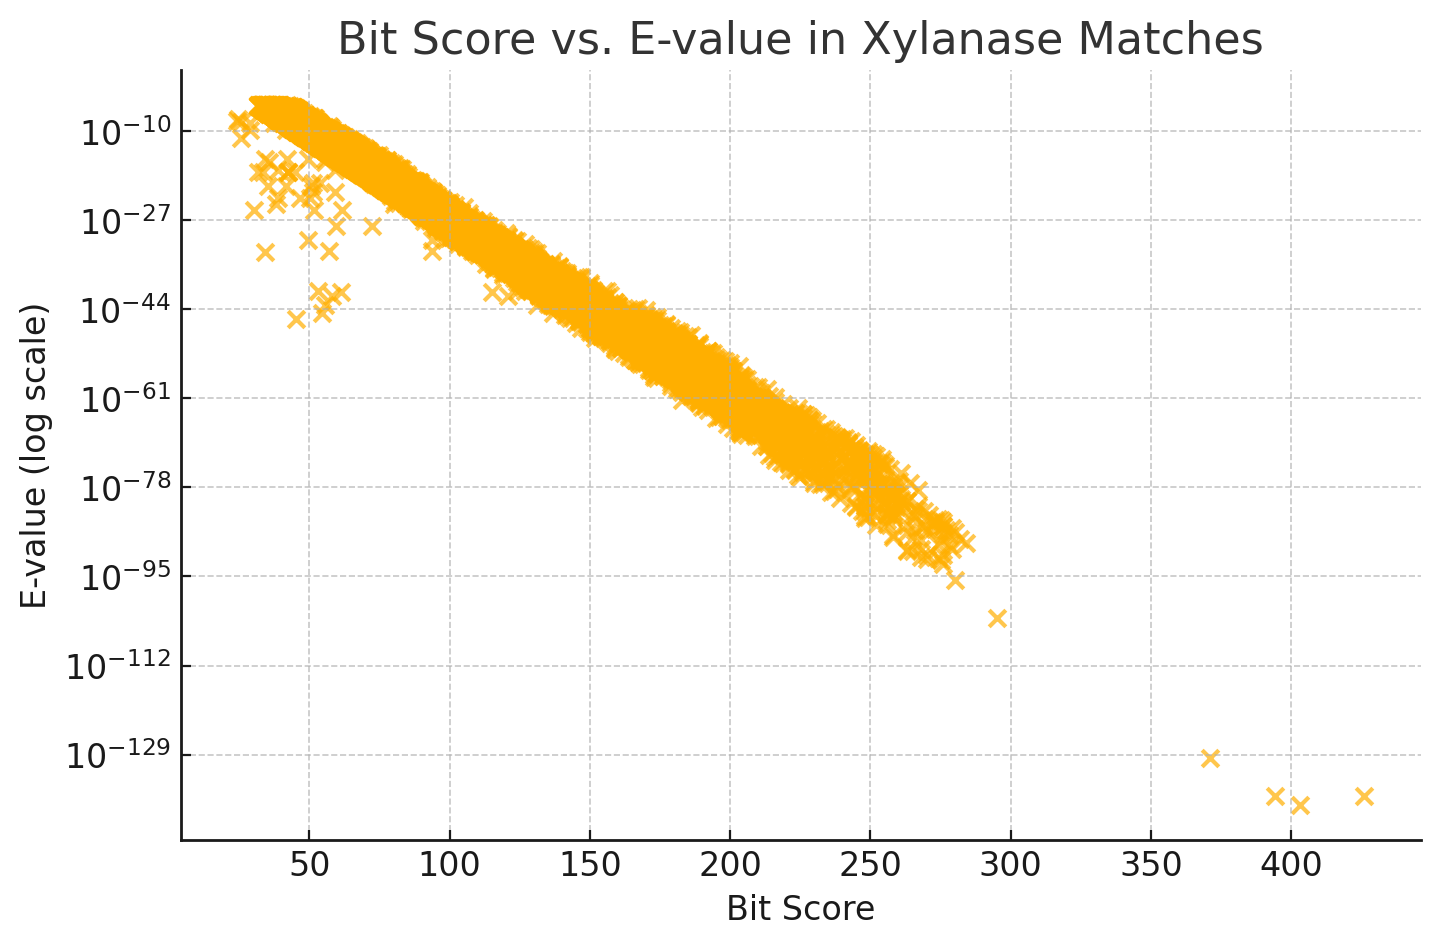
\includegraphics[width=0.8\textwidth]{images/bitscore_evalue.png} % Replace with your image file
                \caption{نمودار پراکندگی: امتیاز بیت در مقابل e-value}
                \label{fig:bitscore_evalue}
            \end{figure}
            نمودار پراکندگی: امتیاز بیت در مقابل e-value\\
            مشاهدات:
            \begin{itemize}
                \item امتیاز بیت بالا با مقادیر E کمتر مطابقت دارد، که تطابق قوی و معنی دار آماری را تایید می کند.
                \item برخی از توالی‌ها امتیاز بیت‌های متوسطی را نشان می‌دهند، اما همچنان دارای مقادیر E پایین هستند، به این معنی که تا حدی با زایلانازهای شناخته شده مطابقت دارند، اما ممکن است انواع متفاوتی باشند.
            \end{itemize}
            مفاهیم:
            \begin{itemize}
                \item امتیاز بیت بالا و ارزش E پایین $\leftarrow$ کاندیدهای قوی زایلاناز ارزش بررسی بیشتر را دارند.
                \item امتیاز بیت متوسط ​​و ارزش E پایین $\leftarrow$ آنزیم های جدید بالقوه با شباهت جزئی به زایلانازهای شناخته شده.
            \end{itemize}
            \item 
            \begin{figure}[H]
                \centering
                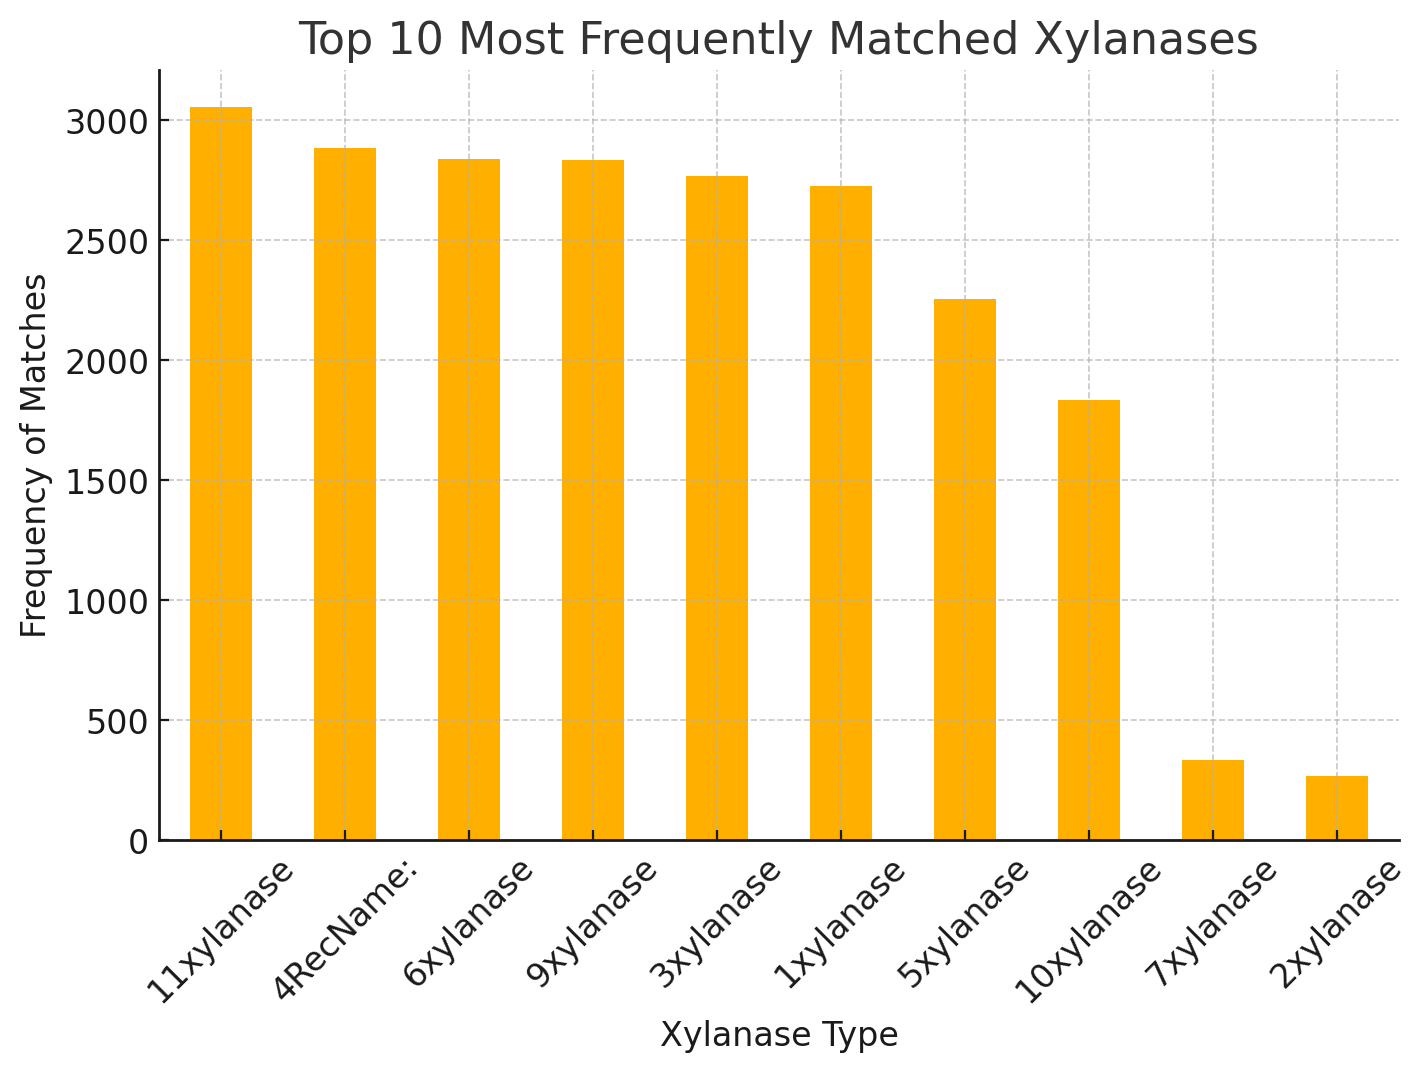
\includegraphics[width=0.8\textwidth]{images/top_freq.png} % Replace with your image file
                \caption{نمودار میله ای: 10 زایلاناز برتر که بیشترین تطبیق را دارند}
                \label{fig:top_freq}
            \end{figure}
            نمودار میله ای: 10 زایلاناز برتر که بیشترین تطبیق را دارند\\
            مشاهدات:
            \begin{itemize}
                \item برخی از آنزیم‌های زایلاناز بیشتر در چند شاخه ظاهر می‌شوند، که نشان می‌دهد در متاژنوم شکمبه فراوان هستند.
                \item بیشترین تطابق زایلانازها احتمالاً متعلق به خانواده های آنزیمی بسیار حفاظت شده در میکروبیوم شکمبه است.
            \end{itemize}
            مفاهیم:
            \begin{itemize}
                \item انواع زایلاناز غالب ممکن است از نظر عملکردی در تخریب لیگنوسلولز در شکمبه مهم باشند.
                \item زایلانازهایی که کمتر مطابقت دارند ممکن است آنزیم های کمیاب یا جدید باشند که ارزش توصیف بیشتر را دارند.
            \end{itemize}
        \end{enumerate}

        هیستوگرام توزیع درصد هویت (شکل 1) نشان می دهد که اکثر کانتیگ ها 30-60 درصد هویت با زایلانازهای شناخته شده دارند. این نشان می دهد که در حالی که برخی از نامزدها ارتباط نزدیکی با زایلانازهای مرجع دارند، برخی دیگر ممکن است انواع جدیدی را ارائه دهند. نمودار پراکندگی بیت امتیاز در مقابل ارزش E (شکل 2) نشان می دهد که امتیاز بیت بالاتر با مقادیر E پایین تر همبستگی دارد و تأیید می کند که این توالی ها از نظر آماری با زایلانازهای شناخته شده مطابقت دارند.

        از طریق جستجوهای مبتنی بر شباهت، مجموعه‌ای از توالی‌های کاندید زایلاناز را از متاژنوم شکمبه شناسایی کردیم. این توالی ها بر اساس درصد هویت، طول هم ترازی و اهمیت آماری فیلتر شدند تا از انتخاب قابل اعتماد اطمینان حاصل شود. مرحله بعدی شامل خوشه‌بندی این توالی‌ها برای حذف افزونگی و انتخاب توالی‌های نماینده برای مدل‌سازی منطقه حفاظت‌شده است. این به ما این امکان را می دهد که انتخاب کاندیدهای زایلاناز پایدار در برابر حرارت را برای کاربردهای صنعتی اصلاح کنیم.
